\documentclass[14pt]{extbook}
\usepackage{multicol, enumerate, enumitem, hyperref, color, soul, setspace, parskip, fancyhdr} %General Packages
\usepackage{amssymb, amsthm, amsmath, latexsym, units, mathtools} %Math Packages
\everymath{\displaystyle} %All math in Display Style
% Packages with additional options
\usepackage[headsep=0.5cm,headheight=12pt, left=1 in,right= 1 in,top= 1 in,bottom= 1 in]{geometry}
\usepackage[usenames,dvipsnames]{xcolor}
\usepackage{dashrule}  % Package to use the command below to create lines between items
\newcommand{\litem}[1]{\item#1\hspace*{-1cm}\rule{\textwidth}{0.4pt}}
\pagestyle{fancy}
\lhead{Makeup Progress Quiz 2}
\chead{}
\rhead{Version B}
\lfoot{5763-3522}
\cfoot{}
\rfoot{Spring 2021}
\begin{document}

\begin{enumerate}
\litem{
Choose the graph of the equation below.\[ f(x) = \sqrt{x - 6} - 6 \]\begin{enumerate}[label=\Alph*.]
\begin{multicols}{2}\item 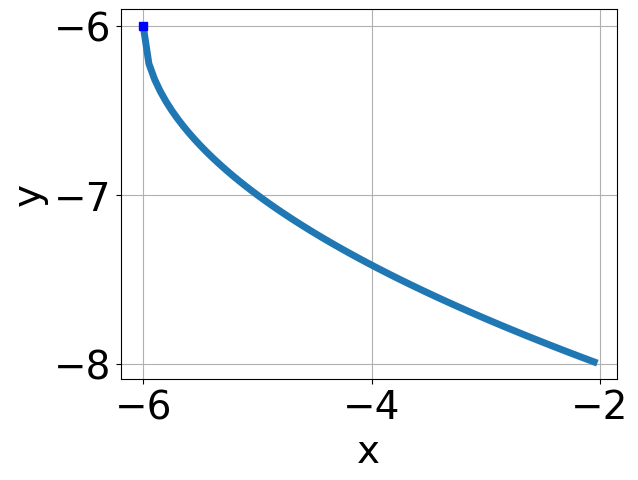
\includegraphics[width = 0.3\textwidth]{../Figures/radicalEquationToGraphAB.png}\item 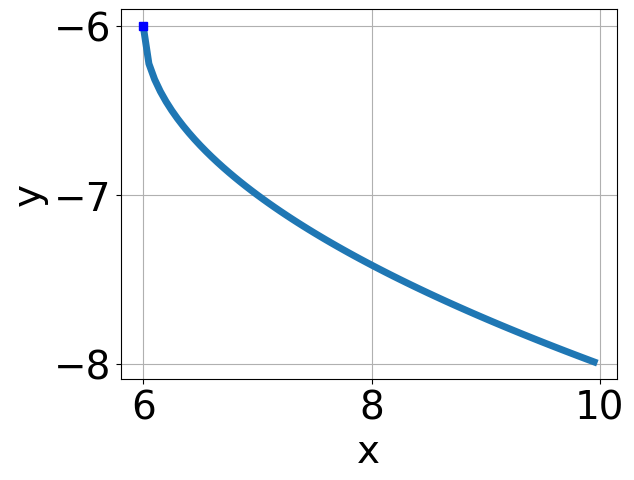
\includegraphics[width = 0.3\textwidth]{../Figures/radicalEquationToGraphBB.png}\item 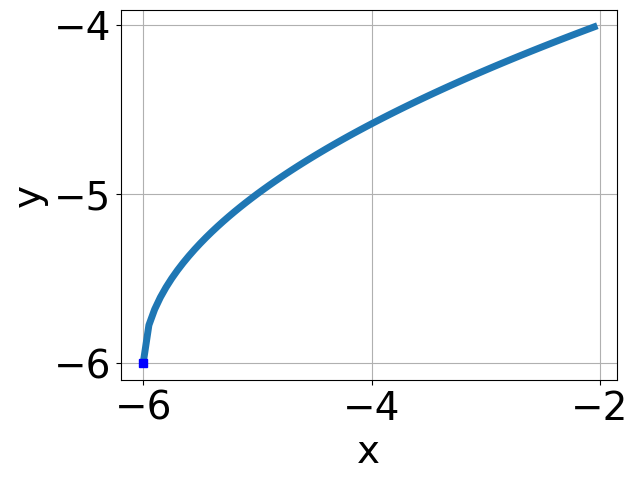
\includegraphics[width = 0.3\textwidth]{../Figures/radicalEquationToGraphCB.png}\item 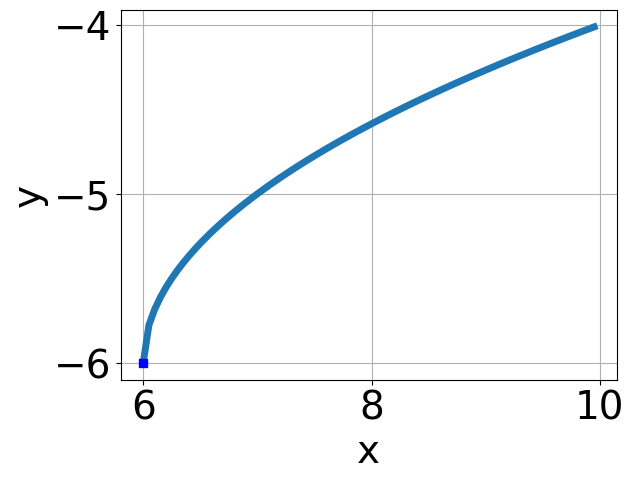
\includegraphics[width = 0.3\textwidth]{../Figures/radicalEquationToGraphDB.png}\end{multicols}\item None of the above.
\end{enumerate} }
\litem{
Choose the equation of the function graphed below.
\begin{center}
    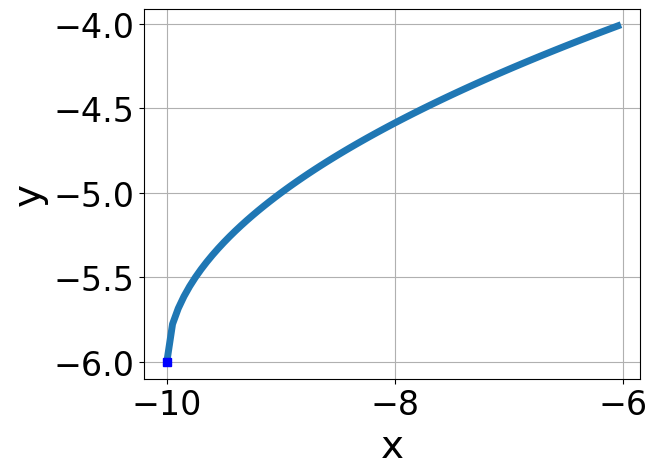
\includegraphics[width=0.5\textwidth]{../Figures/radicalGraphToEquationB.png}
\end{center}
\begin{enumerate}[label=\Alph*.]
\item \( f(x) = - \sqrt{x - 10} - 6 \)
\item \( f(x) = - \sqrt{x + 10} - 6 \)
\item \( f(x) = \sqrt{x - 10} - 6 \)
\item \( f(x) = \sqrt{x + 10} - 6 \)
\item \( \text{None of the above} \)

\end{enumerate} }
\litem{
Choose the graph of the equation below.\[ f(x) = \sqrt{x - 6} - 3 \]\begin{enumerate}[label=\Alph*.]
\begin{multicols}{2}\item 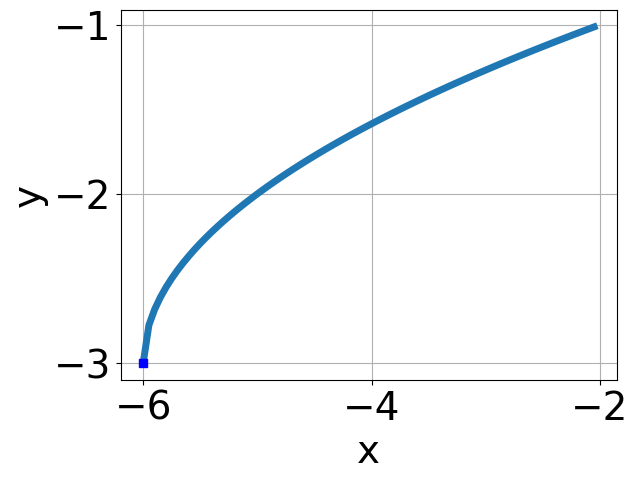
\includegraphics[width = 0.3\textwidth]{../Figures/radicalEquationToGraphCopyAB.png}\item 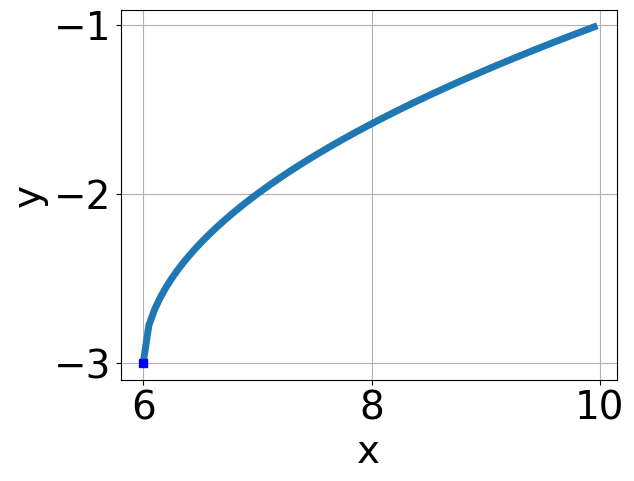
\includegraphics[width = 0.3\textwidth]{../Figures/radicalEquationToGraphCopyBB.png}\item 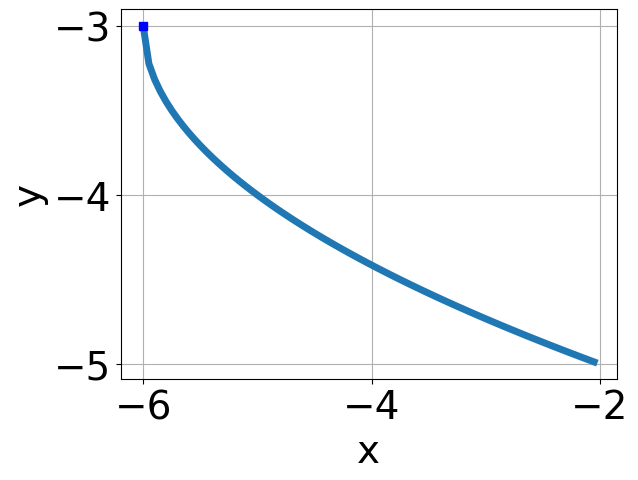
\includegraphics[width = 0.3\textwidth]{../Figures/radicalEquationToGraphCopyCB.png}\item 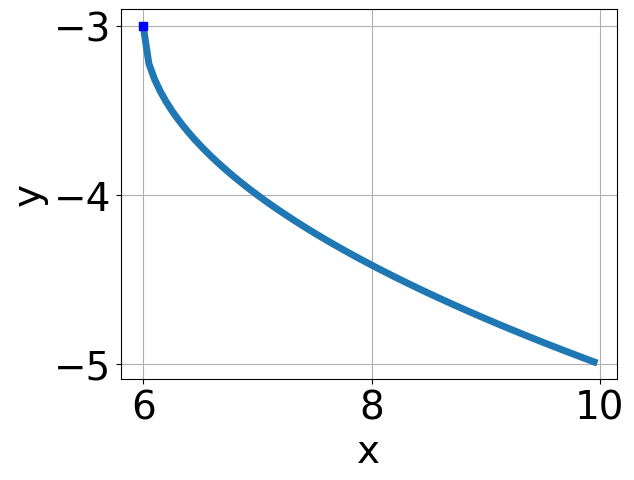
\includegraphics[width = 0.3\textwidth]{../Figures/radicalEquationToGraphCopyDB.png}\end{multicols}\item None of the above.
\end{enumerate} }
\litem{
What is the domain of the function below?\[ f(x) = \sqrt[4]{5 x - 4} \]\begin{enumerate}[label=\Alph*.]
\item \( (-\infty, a], \text{where } a \in [0.05, 0.8] \)
\item \( (-\infty, a], \text{where } a \in [1.14, 1.4] \)
\item \( (-\infty, \infty) \)
\item \( [a, \infty), \text{where } a \in [0.97, 1.48] \)
\item \( [a, \infty), \text{ where } a \in [0.75, 1.15] \)

\end{enumerate} }
\litem{
Solve the radical equation below. Then, choose the interval(s) that the solution(s) belongs to.\[ \sqrt{-14 x^2 - 18} - \sqrt{-48 x} = 0 \]\begin{enumerate}[label=\Alph*.]
\item \( x_1 \in [-0.11, 0.96] \text{ and } x_2 \in [3,6] \)
\item \( x \in [-0.11,0.96] \)
\item \( x \in [1.77,3.24] \)
\item \( \text{All solutions lead to invalid or complex values in the equation.} \)
\item \( x_1 \in [-1.17, -0.01] \text{ and } x_2 \in [-3,-1] \)

\end{enumerate} }
\litem{
What is the domain of the function below?\[ f(x) = \sqrt[6]{7 x - 5} \]\begin{enumerate}[label=\Alph*.]
\item \( [a, \infty), \text{ where } a \in [0.22, 0.75] \)
\item \( (-\infty, a], \text{where } a \in [-1.13, 0.94] \)
\item \( [a, \infty), \text{where } a \in [0.85, 1.88] \)
\item \( (-\infty, a], \text{where } a \in [0.83, 1.66] \)
\item \( (-\infty, \infty) \)

\end{enumerate} }
\litem{
Solve the radical equation below. Then, choose the interval(s) that the solution(s) belongs to.\[ \sqrt{-48 x^2 - 36} - \sqrt{-96 x} = 0 \]\begin{enumerate}[label=\Alph*.]
\item \( x_1 \in [-1.61, 0.05] \text{ and } x_2 \in [-4.5,-0.5] \)
\item \( x \in [-0.25,0.57] \)
\item \( \text{All solutions lead to invalid or complex values in the equation.} \)
\item \( x_1 \in [-0.25, 0.57] \text{ and } x_2 \in [-0.5,4.5] \)
\item \( x \in [1.43,1.59] \)

\end{enumerate} }
\litem{
Solve the radical equation below. Then, choose the interval(s) that the solution(s) belongs to.\[ \sqrt{4 x - 7} - \sqrt{6 x - 6} = 0 \]\begin{enumerate}[label=\Alph*.]
\item \( x \in [-2.5,0.5] \)
\item \( x \in [-7.5,-3.5] \)
\item \( x_1 \in [-2.5, 0.5] \text{ and } x_2 \in [-0.25,8.75] \)
\item \( x_1 \in [1, 7] \text{ and } x_2 \in [-0.25,8.75] \)
\item \( \text{All solutions lead to invalid or complex values in the equation.} \)

\end{enumerate} }
\litem{
Solve the radical equation below. Then, choose the interval(s) that the solution(s) belongs to.\[ \sqrt{-4 x + 8} - \sqrt{8 x + 2} = 0 \]\begin{enumerate}[label=\Alph*.]
\item \( x_1 \in [-0.8, -0.07] \text{ and } x_2 \in [2,5] \)
\item \( x_1 \in [0.32, 0.63] \text{ and } x_2 \in [2,5] \)
\item \( x \in [0.58,0.97] \)
\item \( x \in [0.32,0.63] \)
\item \( \text{All solutions lead to invalid or complex values in the equation.} \)

\end{enumerate} }
\litem{
Choose the equation of the function graphed below.
\begin{center}
    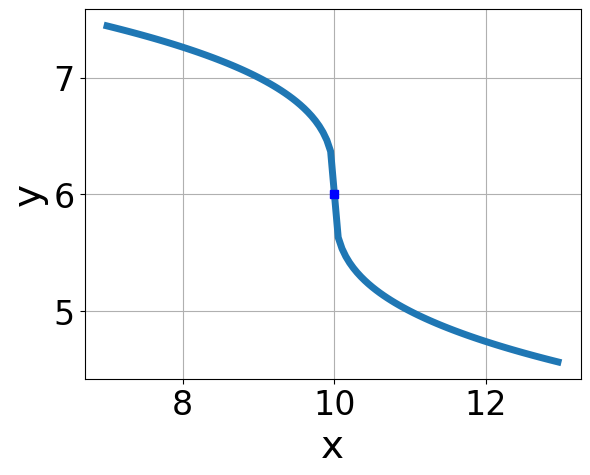
\includegraphics[width=0.5\textwidth]{../Figures/radicalGraphToEquationCopyB.png}
\end{center}
\begin{enumerate}[label=\Alph*.]
\item \( f(x) = \sqrt{x - 10} + 6 \)
\item \( f(x) = - \sqrt{x + 10} + 6 \)
\item \( f(x) = - \sqrt{x - 10} + 6 \)
\item \( f(x) = \sqrt{x + 10} + 6 \)
\item \( \text{None of the above} \)

\end{enumerate} }
\end{enumerate}

\end{document}